\documentclass{report}
\usepackage{polski}
\usepackage[utf8]{inputenc}
\usepackage{float}
\usepackage{graphicx}
\usepackage{caption}
\usepackage{subcaption}
\usepackage{ragged2e}
\usepackage{blindtext}
\usepackage{hyperref}
\usepackage{amssymb}
\graphicspath{ {../plots/} }
\begin{document}
\author{Jakub Ogrodowczyk}
\AddToHook{cmd/section/before}{\clearpage}

\section*{Zadanie 1}
Ciągi bitowe generowałem za pomocą języka C++. Jako gorszy generator (LCG)
użyłem funkcji rand(), a jako lepszy implementacji Mersenne Twister z biblioteki
standardowej C++. Zgodnie z https://nvlpubs.nist.gov/nistpubs/Legacy/SP/nistspecialpublication800-22r1a.pdf
aby wszystkie testy poprawnie działały potrzebujemy co najmniej 1.35 mln bitów.
Ja generowałem ich 1.5 mln.
\begin{figure}[H]
    \centering
    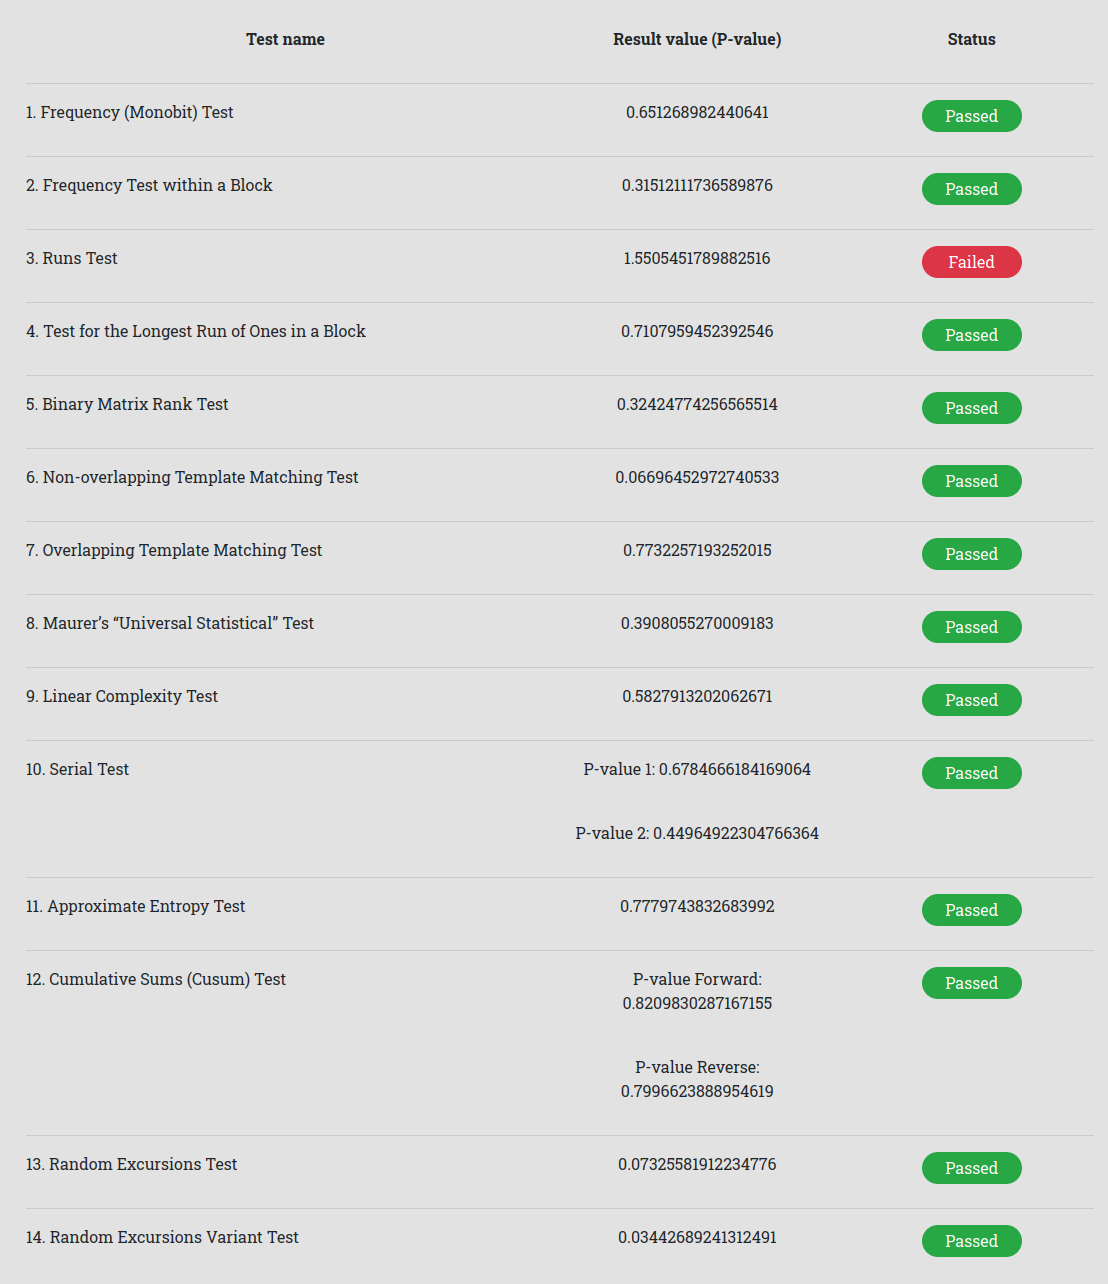
\includegraphics[scale=0.4]{../gorszy_generator.png}
    \caption[Example .]{Wyniki testu NIST dla generatora LCG}
    \label{plotB}
\end{figure}
Jak widać gorszy generator poradził sobie względnie dobrze, nie przeszedł
tylko testu nr 3. Test ten sprawdza czy dany generator wystarczająco często
oscyluje między 0, a 1, tzn. czy ilość sekwencji zer i jedynek o różnych
długościach jest zgodna z oczekiwaną. Generator LCG cechuje się tym, że
generuje liczby równomiernie na całym swoim przedziale, w przypadku funkcji
rand() w C jest to przedział [0,\textrm{RAND\_MAX}]. Jeśli więc chcemy wygenerować
liczby całkowite na przedziale [a,b) to będą one rozłożone równomiernie tylko wtedy,
gdy \(b\mid\textrm{RAND\_MAX}\). Na moim komputerze \(\textrm{RAND\_MAX} = 2147483647\).
Oczywiście \(2 \nmid 2147483647\), a więc generator ten nie będzie dobry w generowaniu
losowych ciągów bitowych.
\begin{figure}[H]
    \centering
    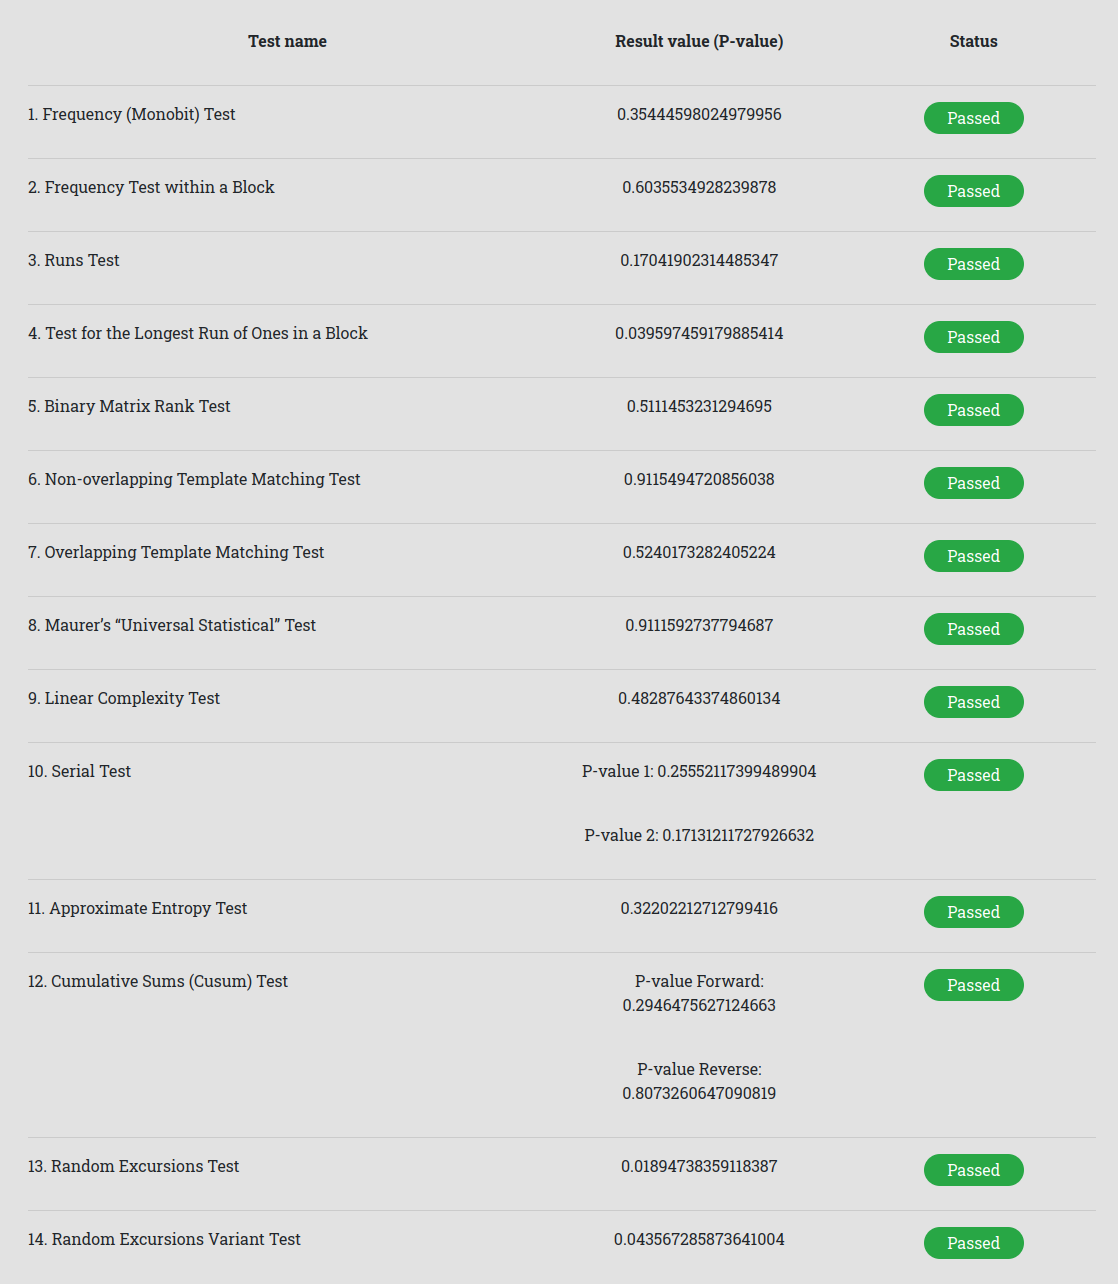
\includegraphics[scale=0.5]{../lepszy_generator.png}
    \caption[Example .]{Wyniki testu NIST dla generatora Mersenne Twister}
    \label{plotB}
\end{figure}
Generator Mersenne Twister zgodnie z oczekiwaniami przeszedł wszystkie testy.

\begin{figure}[H]
    \centering
    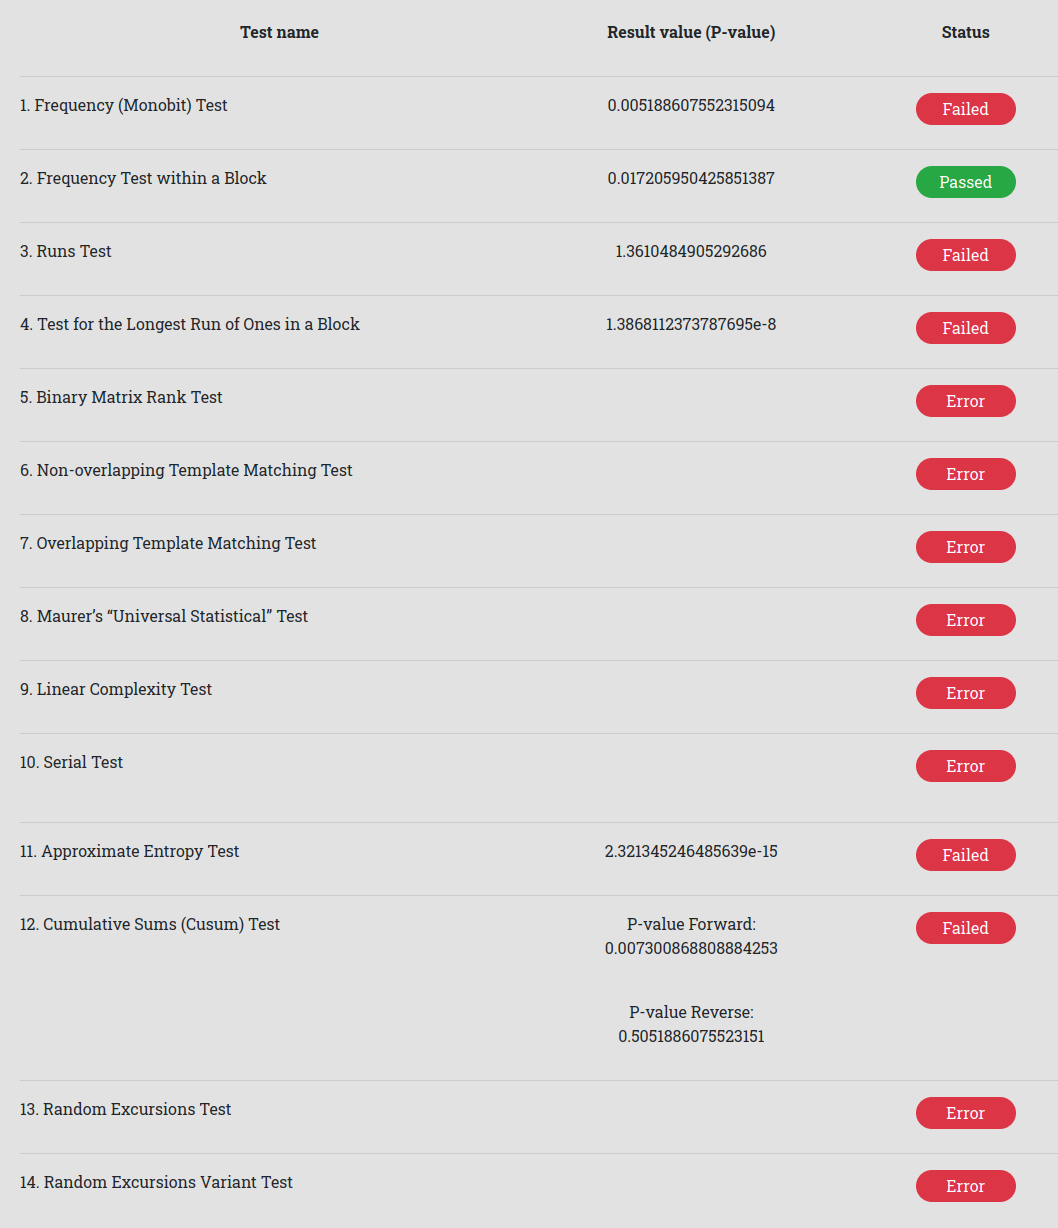
\includegraphics[scale=0.5]{../imie.png}
    \caption[Example .]{Wyniki testu NIST dla generatora hashu SHA1 mojego nazwiska}
    \label{plotB}
\end{figure}
Oczywiście, tak jak pisałem wyżej, hash SHA1 jest zbyt krótki (322 bitów) aby
przejść testy, do których wymagane jest 1.3 mln bitów, więc hash mojego nazwiska
przeszedł tylko jeden test, podczas gdy na większości miał error.

\section*{Zadanie 2}
Poniżej są wykresy wygenerowane za pomocą symulacji napisanej w języku python.
Symulacja polega na niezależnym wygenerowaniu 10000 razy zmiennej S(N),
zliczeniu wystąpień poszczególnych wartości, a następnie wygenerowaniu dystrybuanty.
\begin{figure}[H]
    \centering
    \begin{subfigure}{.5\textwidth}
      \centering
      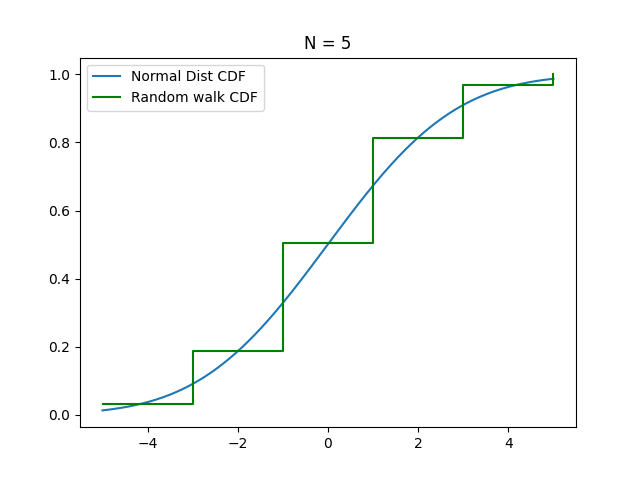
\includegraphics[width=1.1\linewidth]{plotN5.png}
      \caption{N = 5}
      \label{fig:plotbnfunc1}
    \end{subfigure}%
    \begin{subfigure}{.5\textwidth}
      \centering
      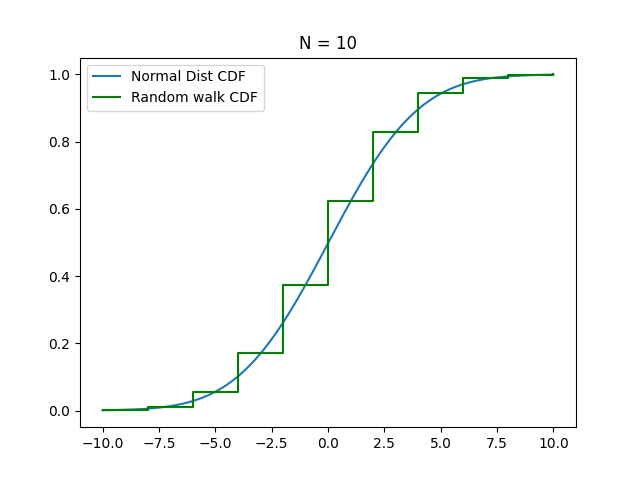
\includegraphics[width=1.1\linewidth]{plotN10.png}
      \caption{N = 10}
      \label{fig:plotbnfunc2}
    \end{subfigure}
    \begin{subfigure}{.5\textwidth}
        \centering
        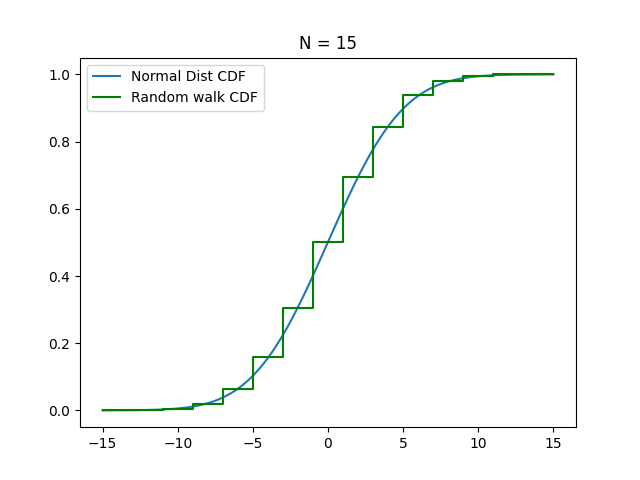
\includegraphics[width=1.1\linewidth]{plotN15.png}
        \caption{N = 15}
        \label{fig:plotbnfunc1}
    \end{subfigure}%
    \begin{subfigure}{.5\textwidth}
        \centering
        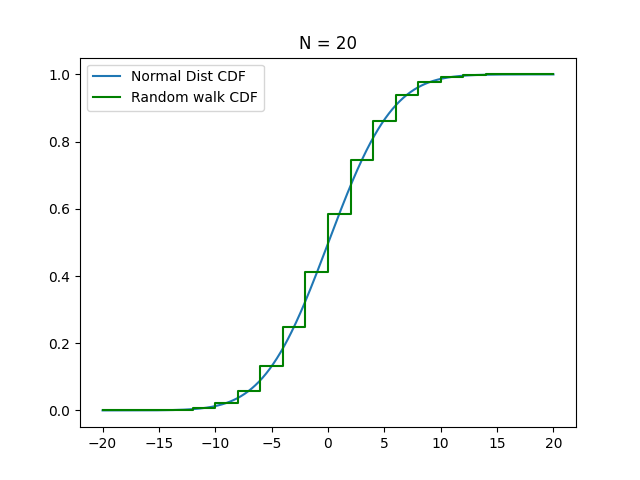
\includegraphics[width=1.1\linewidth]{plotN20.png}
        \caption{N = 20}
        \label{fig:plotbnfunc1}
    \end{subfigure}%
    \caption{Wykresy przedstawiające wyniki dla \(N\in[5,10,15,20] \)}
    \label{fig:bn}
\end{figure}

\begin{figure}[H]
    \centering
    \begin{subfigure}{.5\textwidth}
      \centering
      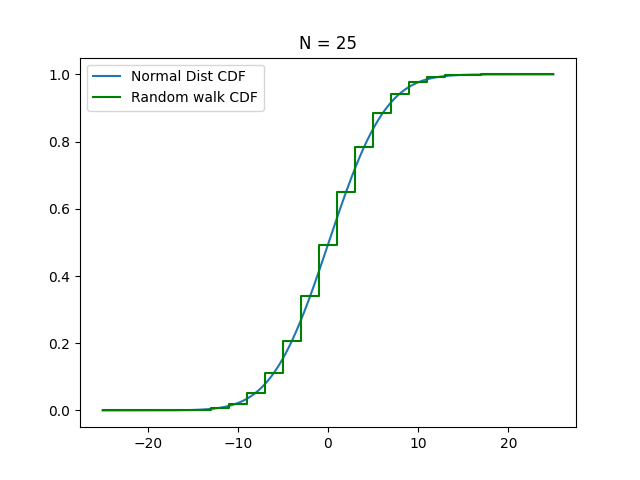
\includegraphics[width=1.1\linewidth]{plotN25.png}
      \caption{N = 25}
      \label{fig:plotbnfunc1}
    \end{subfigure}%
    \begin{subfigure}{.5\textwidth}
      \centering
      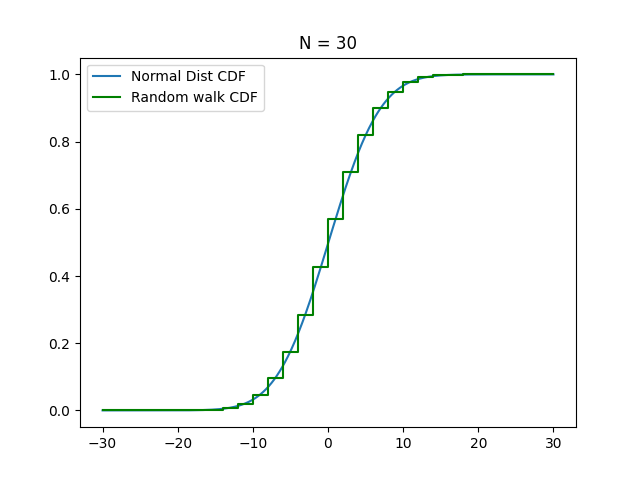
\includegraphics[width=1.1\linewidth]{plotN30.png}
      \caption{N = 30}
      \label{fig:plotbnfunc2}
    \end{subfigure}
    \caption{Wykresy przedstawiające wyniki dla \(N\in[25,30] \)}
    \label{fig:bn}
\end{figure}

\begin{figure}[htp]
    \centering
    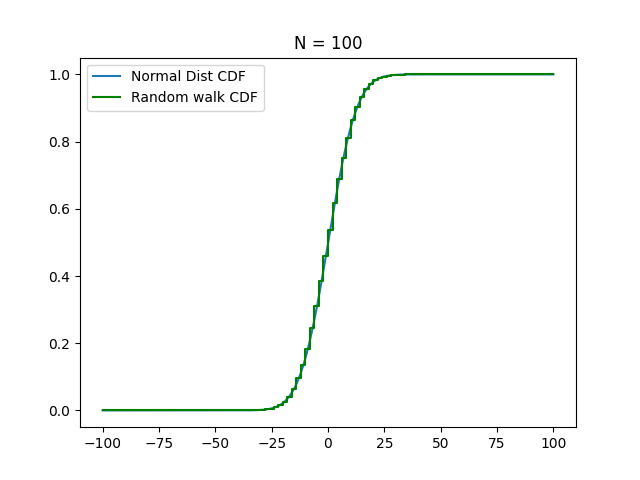
\includegraphics[scale=0.5]{plotN100.png}
    \caption[Example .]{Wykres przedstawiający wyniki eksperymentu dla N = 100}
    \label{plotB}
\end{figure}

Zgodnie z intuicją, wraz z rosnącymi wartościami N symulacja "random walk"
coraz dokładniej aproksymuje rozkład normalny.

\section*{Zadanie 3}

\begin{figure}[htp]
    \centering
    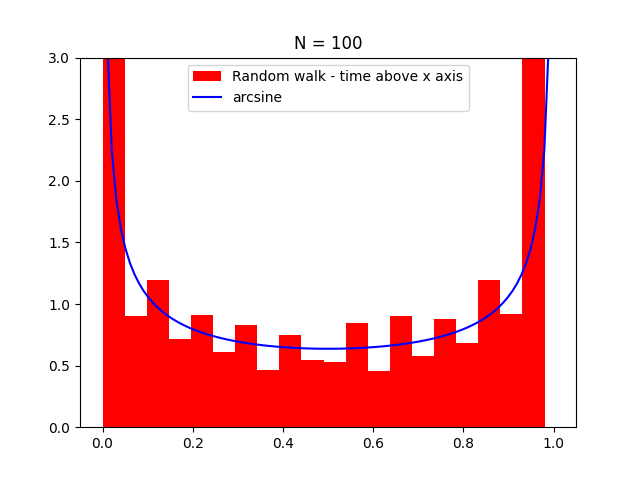
\includegraphics[scale=0.5]{plotZad3N100.png}
    \caption[Example .]{Wykres przedstawiający wyniki eksperymentu dla N = 100}
    \label{plotB}
\end{figure}

\begin{figure}[htp]
    \centering
    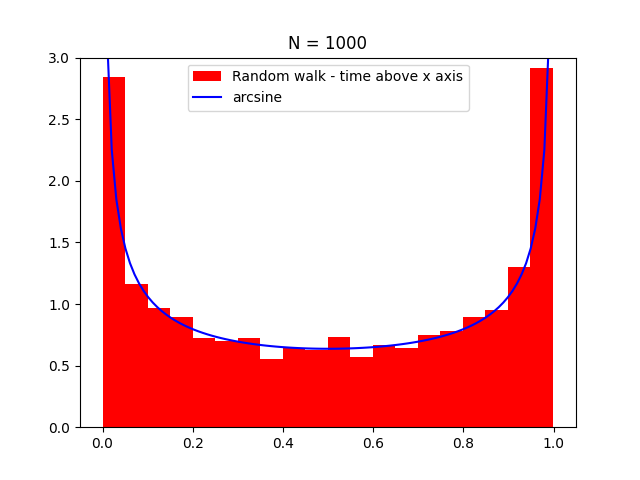
\includegraphics[scale=0.5]{plotZad3N1000.png}
    \caption[Example .]{Wykres przedstawiający wyniki eksperymentu dla N = 1000}
    \label{plotB}
\end{figure}

\begin{figure}[H]
    \centering
    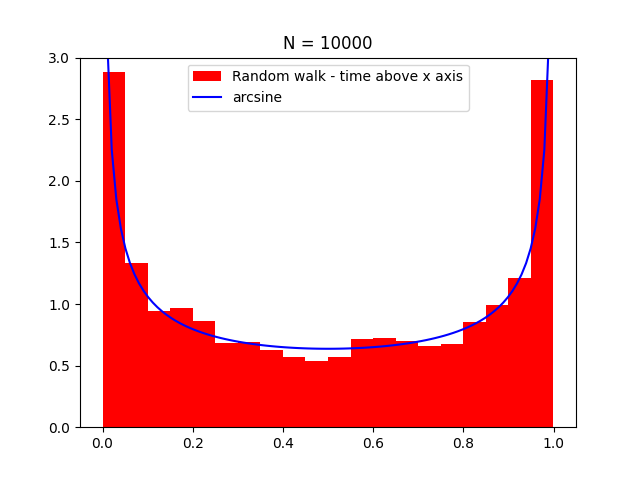
\includegraphics[scale=0.7]{plotZad3N10000.png}
    \caption[Example .]{Wykres przedstawiający wyniki eksperymentu dla N = 10000}
    \label{plotB}
\end{figure}

Nasz eksperyment wraz z rosnącym N coraz ściślej przybliża rozkład arcsinusa.

\end{document}